\documentclass[../main.tex]{subfiles}

\begin{document}

\problem{5}

Consider the bar loaded as shown in figure \ref{}.

Assume \(E=200\,\unit{\giga\pascal}\) and that the bar is fixed at both ends.

\begin{enumerate}[label=\alph*)]
    \item Construct a 1D linear bar finite element model of the bar. \textit{Use two elements in each section of the bar (4 elements in total).} \underline{Label all nodes and elements}.
    \item Write the global system of equations \([K]\{d\} = \{R\}\).
    \item Apply the boundary conditions to this global system of equations and solve for \(\{d\}\).
    \item Plot the displacements \(u(x)\) vs. \(x\) for the entire bar.
    \item What are the reaction forces at the two ends?
\end{enumerate}

\problempart{a}

Figure \ref{fea_bar} shows the 1D linear bar finite element model of the bar given in the problem statement.
The model has 4 elements and 5 nodes, with the known tractions, forces, and boundary conditions shown in the figure.

\begin{figure}[h!]
    \centering
    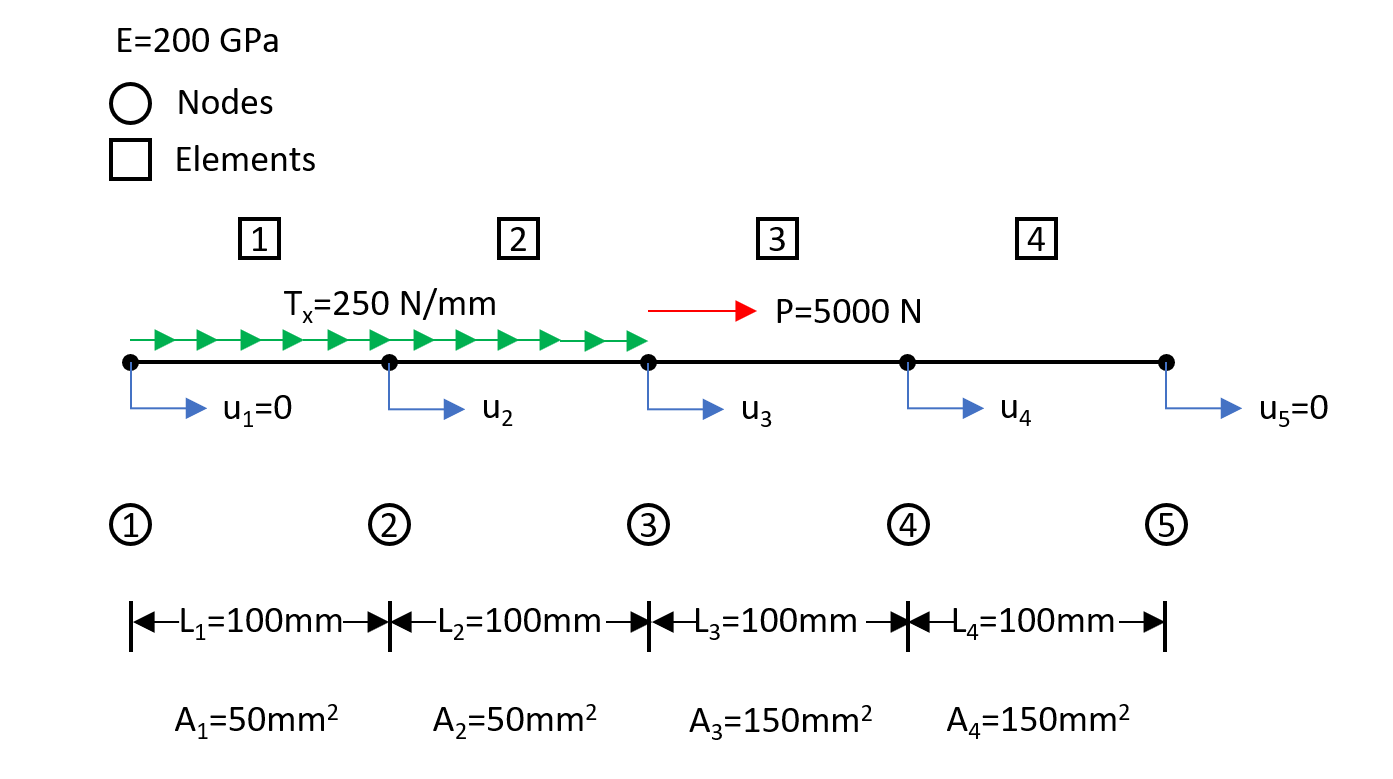
\includegraphics[scale=0.45]{../../images/problem_5/5elementbar.png}
    \caption{1D linear bar finite element model of bar.}
    \label{fea_bar}
\end{figure}

\problempart{b}

Let \(k_i = \frac{EA_i}{L_i}\).
We assemble a local stiffness matrix \([K_i\)] for each element \(i\) as shown below:

\[
    [K_1] = \mqty[k_1 & -k_1\\ -k_1 & k_1]
\]

\[
    [K_2] = \mqty[k_2 & -k_2\\ -k_2 & k_2]
\]

\[
    [K_3] = \mqty[k_3 & -k_3\\ -k_3 & k_3]
\]

\[
    [K_4] = \mqty[k_4 & -k_4\\ -k_4 & k_4]
\]

Through superposition we combine the local stiffness matrices into a global stiffness matrix, \([K]\):

\[
    \begin{aligned}
    [K] = 
    &
    \mqty[
        k_1 & -k_1 & 0 & 0 & 0\\
        -k_1 & k_1 & 0 & 0 & 0\\
        0 & 0 & 0 & 0 & 0 \\
        0 & 0 & 0 & 0 & 0 \\
        0 & 0 & 0 & 0 & 0
    ]
    +
    \mqty[
        0 & 0 & 0 & 0 & 0\\
        0 & k_2 & -k_2 & 0 & 0\\
        0 & -k_2 & k_2 & 0 & 0 \\
        0 & 0 & 0 & 0 & 0 \\
        0 & 0 & 0 & 0 & 0
    ]
    +  \\
    &
    \mqty[
        0 & 0 & 0 & 0 & 0\\
        0 & 0 & 0 & 0 & 0\\
        0 & 0 & k_3 & -k_3 & 0 \\
        0 & 0 & -k_3 & k_3 & 0 \\
        0 & 0 & 0 & 0 & 0
    ]
    +
    \mqty[
        0 & 0 & 0 & 0 & 0\\
        0 & 0 & 0 & 0 & 0\\
        0 & 0 & 0 & 0 & 0 \\
        0 & 0 & 0 & k_4 & -k_4 \\
        0 & 0 & 0 & -k_4 & k_4
    ]
    \end{aligned}
\]

\[
    [K] =
    \mqty[
        k_1 & -k_1 & 0 & 0 & 0\\
        -k_1 & k_1+k_2 & -k_2 & 0 & 0\\
        0 & -k_2 & k_2+k_3 & -k_3 & 0 \\
        0 & 0 & -k_3 &k_3 + k_4 & -k_4 \\
        0 & 0 & 0 & -k_4 & k_4
    ]
\]

Next, we assemble our displacement vector, noting that \(d_1 = d_5 = 0\):

\[
    \{d\} = 
    \begin{Bmatrix}
        d_1 \\ d_2 \\ d_3 \\d_4 \\d_5
    \end{Bmatrix}
    =
    \begin{Bmatrix}
        0 \\ d_2 \\ d_3 \\d_4 \\ 0
    \end{Bmatrix}
\]

Then, the vector of applied forces:

\[
    \{r\} = 
    \begin{Bmatrix}
        F_1 \\ F_2 \\ F_3 \\ F_4 \\ F_5
    \end{Bmatrix}
\]

\(F_1\) and \(F_5\) are unknown because we know that the displacements at both boundaries are 0.
The applied forces at nodes 2-4 are outlined below:

\[  
    F_2 = T_x * L_1  
\]

\[
    F_3 = T_x * (L_1 + L_2) + P
\]

\[
    F_4 = P
\]

\[
    \{r\} = 
    \begin{Bmatrix}
        F_1 \\ T_x * L_1 \\ T_x * (L_1 + L_2) + P \\ P \\ F_5
    \end{Bmatrix}
    =
    \begin{Bmatrix}
        F_1 \\ 30000 \\ 55000 \\ 5000 \\ F_5
    \end{Bmatrix}
\]

The global system of equations \([K]\{d\} = \{r\}\):

\[
    \boxed{
    \mqty[
        k_1 & -k_1 & 0 & 0 & 0\\
        -k_1 & k_1+k_2 & -k_2 & 0 & 0\\
        0 & -k_2 & k_2+k_3 & -k_3 & 0 \\
        0 & 0 & -k_3 &k_3 + k_4 & -k_4 \\
        0 & 0 & 0 & -k_4 & k_4
    ]
    \begin{Bmatrix}
        0 \\ d_2 \\ d_3 \\d_4 \\ 0
    \end{Bmatrix}
    =
    \begin{Bmatrix}
        F_1 \\ 30000 \\ 55000 \\ 5000 \\ F_5
    \end{Bmatrix}
    }
\]

\problempart{c}

Substituting in given values and solving in MATLAB yields the following for \(\{d\}\):

\[
    \boxed{\{d\} =     
    \begin{Bmatrix}
        d_1 \\ d_2 \\ d_3 \\d_4 \\d_5
    \end{Bmatrix}
    =
    \begin{Bmatrix}
        0 \\ 0.3313 \\ 0.3625 \\ 0.1896 \\ 0
    \end{Bmatrix} \, \unit{\milli\meter}}
\]

\problempart{d}

some ldkjfhsdlkfjhdslkjfhdskljfhdskl \textbf{MORE HERE MORE HERE MORE HERE}
dfgdf
dfgdf
dfgdf
\begin{figure}[h!]
    \centering
    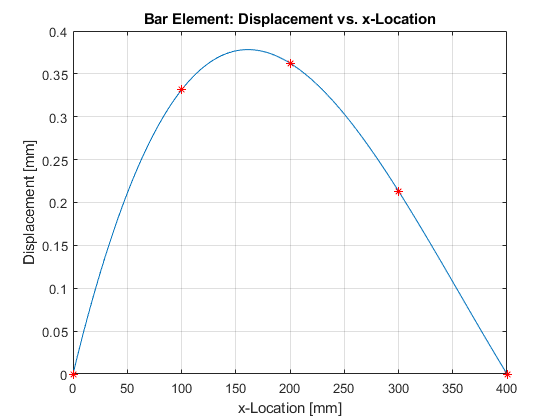
\includegraphics[scale=1]{../../images/problem_5/u_vs_x.png}
    \caption{Displacement \(u\) vs. \(x\) location}
    \label{u_vs_x}
\end{figure}

\problempart{e}

Solving the global  \([K]\{d\} = \{r\}\) equation in MATLAB yields the following for \(\{r\}\):

\[
    \{r\} =
    \begin{Bmatrix}
        F_1 \\ F_2 \\ F_3 \\ F_4 \\ F_5
    \end{Bmatrix}
    =
    \begin{Bmatrix}
        -33125 \\ 30000 \\ 55000 \\ 5000 \\ -56875
    \end{Bmatrix}   
    \, \unit{\newton}
\]

The reaction forces at the ends are given by \(F_1\) and \(F_5\):

\[
    \boxed{F_1 = -33125 \, \unit{\newton} \quad \quad F_5 = -56875 \, \unit{\newton}}
\]

\end{document}